% Introduction

% Main chapter title
\chapter{Decoding Algorithm} 

% Change X to a consecutive number; for referencing this chapter elsewhere, use \ref{ChapterX}
\label{Chapter3} 

% This is for the header on each page
\lhead{Chapter 3. \emph{Decoding Algorithms}}  

\section{Message Passing Decoding}


The algorithms used to decode LDPC codes are iterative in nature. In every iteration some information has to be passed through the edge of the bipartite graph (Tanner graph), representing corresponding parity check matrix. Thus these type of iterative algorithm are generally termed as message passing decoding\cite{9}.\\

An equivalent representation of a LDPC parity check matrix is a Tanner graph. A Tanner graph is a bipartite graph. It has two set of nodes. The set that contains code bits is called bit node set. The set containing parity check nodes is call check node set. And the 1s in parity check matrix are represented by connection between a check node and a bit node in the bipartite graph. Notion of Tanner graph was given by Tanner \\
Example:


\[
 H =  \left[ \begin{array} {c|cccccccc} 
  &    B1 &   B2 &   B3 &  B4  &  B5  &  B6  &  B7  &  B8 \\ \hline
c1 &    1  &   1  &   1  &   0  &   0  &   0  &   0  &   0 \\
c2 &    0  &   0  &   0  &   1  &   1  &   1  &   0  &   0 \\ 
c3 &    1  &   0  &   0  &   1  &   0  &   0  &   1  &   0 \\
c4 &    0  &   1  &   0  &   0  &   1  &   0  &   0  &   1 \end{array} \right] 
\]			

\begin{figure}[h!]
\centering
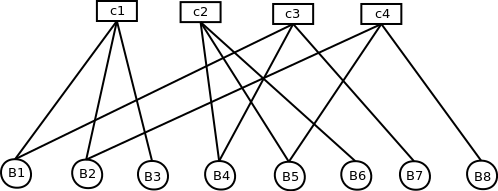
\includegraphics[height=4.5cm,width=10cm]{minSum1}
\caption[Tanner graph]{Tanner graph}
\end{figure}

\subsection{Sum Product Decoding\cite{9}}

The input bit probabilities are called the a priori probabilities.
The bit probabilities returned by the decoder are called the a posteriori probabilities.
For sum-product decoding these probabilities are expressed
as log-likelihood ratios (LLR).
\begin{align} L(x)=log\dfrac{p(x=0)}{p(x=1)}=log\dfrac{1-p(x=1)}{p(x=1)} \end{align}
 If p(x = 0) $>$ p(x = 1) then L(x) is positive.
%The greater the difference between p(x = 0) and p(x = 1), i.e. the more
%sure we are that p(x) = 0, the larger the positive value for L(x), and vic. versa.
%Log Likelihood Ratios are used to represent the metrics for a binary variable x
%by a single value rather than individual probability of being zero and one.
%The sign of L(x) provides the hard decision on x and the magnitude $|L(x)|$ represents
%the reliability of this decision.\\
%LLR based representation has benefit when probabilities
%Rneed to be multiplied LLR need only be added, reducing the implementation complexity.
T%he goal is to achieve maximum a posteriori probability of for each bit. 
The extra information about bit i received
from the parity-check j is called extrinsic information for bit i denoted by $E_{j,i}$. The probability ($P_{j,i}^{ext}$ ) that check j is satisfied when ith bit is one is equal to the probability of having odd number of 1s in the check j other than bit i.
\begin{align} P_{j,i}^{ext} = \dfrac{1}{2}-\dfrac{1}{2} \prod_{i'\in B_j, \ i'\neq i }(1-2P_{i'}^{int})  \end{align}
$P_{i'}^{int}$ is a priori probability of ith bit to be 1. Thus,
\[ E_{(j,i)} =  LLR (P_{j,i}^{ext}) = log \left(
\dfrac{1-P_{j,i}^{ext}}{P_{j,i}^{ext}} 
\right)
\]
\[ E_{(j,i)} = log
\left(
\dfrac{\dfrac{1}{2}+\dfrac{1}{2} \prod_{i'\in B_j \ i'\neq i }(1-2P_{i'}^{int}) }{\dfrac{1}{2}-\dfrac{1}{2} \prod_{i'\in B_j \ i'\neq i }(1-2P_{i'}^{int}) } 
\right)
 \]
Using relationship: $tanh \left(  \dfrac{1}{2}log \left( \dfrac{1-p}{p} \right) \right)=1-2p$;
\[ E_{(j,i)} = log
\left(
\dfrac{\dfrac{1}{2}+\dfrac{1}{2} \prod_{i'\in B_j \ i'\neq i }tanh(M_{j,i'}/2) }{\dfrac{1}{2}-\dfrac{1}{2} \prod_{i'\in B_j \ i'\neq i }tanh(M_{j,i'}/2) } 
\right)
 \]
where 
\[ M_{(j,i')} =  LLR (P_{j,i'}^{int}) = log \left(
\dfrac{1-P_{j,i'}^{int}}{P_{j,i'}^{int}} 
\right)
\]
Alternatively, using the relationship
\[ 2tan^{-1}(p)=log \left( \dfrac{1+p}{1-p} \right) \]
%%%%%%%%%%%%%%%%%%%%%%%%%%%%%%%%%%%%%%%%%%%%%
Thus extrinsic information from check j to bit i is:
\begin{align} E_{(j,i)} = 2tan^{-1} \left( \prod_{i'\in B_j ,\ i'\neq i }tanh(M_{j,i'}/2) \right) \end{align}
Total LLR passed to bit i is
\begin{align} L_i = LLR(P_i^{int}) = r_i + \sum_{j\in A_i} E_{j,i} \end{align}
where $r_i$ is input a priori for bit i.
But, message sent again from bit to check avoid the information which checks already have. Thus,
$M_{j,i}$ is not exactly the extrinsic information, it exclude the message generated by the same check node.\\
\begin{align}  M_{j,i} = \sum_{j'\in A_i j'\neq j} E_{j,i} + r_i \end{align}.\\
%\item %Each bit has access to the input a priori LLR, ri, and the LLRs from every
%connected check node. The total LLR of the i-th bit is the sum of these LLRs
     

After every iteration hard decision is made on the LLR post priori. If code satisfies $Hc^T=0$ then decoding stop else $M_{j,i}$ is found and next iteration is performed.
\subsection{Min Sum Decoding}
The min sum decode algorithm is simplification in the sum product algorithm. \\
For BPSK modulation transmitted $0's$ are represented as $-1s$ and transmitted $1s$ are represented as $1s$. \\
The probability that bit 1 is received 
\begin{align} f_y(y|f=-1) = \dfrac{1}{\sqrt{2\pi\sigma^{2}}} \exp{\dfrac{-(y+1)^2}{2\sigma^2}}
 \end{align}
 

The probability that bit 0 is received 
\begin{align} f_y(y|f=1) = \dfrac{1}{\sqrt{2\pi\sigma^{2}}} \exp{\dfrac{-(y-1)^2}{2\sigma^2}}
 \end{align}
 
Thus getting LLR as:
\begin{align}  LLR = \log\dfrac{f_y(y|f=-1)}{f_y(y|f=1)} = \dfrac{-2y}{\sigma^2}
 \end{align}
 
A priori information on the bit node side is expressed in term of LLR as: 
\begin{align}  aPriori[I] = -4 * C[I] * R * \dfrac{Eb}{No} 
 \end{align}
where C[I] = $i^{th}$ code block, R = code rate and 
$\dfrac{Eb}{No}$ = signal to noise power ratio\\
	
Messages are the information propagating from bit nodes to check nodes.
These are initialized to a priori of their respective bit node.	
\begin{align} message[I][J] = aPriori[I] 
 \end{align}
 
Extrinsic information of a bit node is calculated min sum of all the messages connected to 
	that particular check node. 
\begin{align} |E_{(j,i)}| =  Min_{i'\in B_j \ i'\neq i }|M_{j,i'}|   
 \end{align}

\begin{align} sign({E_{(j,i)}}) =  \prod_{i'\in B_j \ i'\neq i }sign(M_{j,i'})   
 \end{align}
 
A posteriori probabilities are the output bit probabilities.
These are used to modify the code block after every iteration.

\begin{align}  aPosteriori[I] = \sum_{j\in A_i} E_{j,i} + aPriori[I] 
 \end{align}
	
Then hard decision is taken on the a posteriori information, that represent the decoded code block.
If decoded code block satisfies $c*H^{T} = 0 $, then decoding stops. Else messages are updated and transmitted back to start the next iteration of decoding.
\begin{align}   message_{(j,i)} = aPosteriori[i] - E_{(j,i)}  
 \end{align}	


